\documentclass{snedecorbeamer}

\usepackage{natbib}

\usetikzlibrary{positioning,decorations.pathreplacing,quotes,overlay-beamer-styles}

\graphicspath{{inc/}}

\begin{document}

% Title page -------------------------------------------------------------------
\title{Automatic Dynamic Relevance Determination}
\subtitle{A methodology for Gaussian process regression\\
  with high-dimensional functional inputs}
\author{Luis Damiano}
\institute{Iowa State University\\
  Department of Statistics}
\date{October 6, 2022}

\begin{frame}
  \titlepage{}
\end{frame}

% Welcome message --------------------------------------------------------------
\begin{frame}
  \frametitle{Welcome to my prelim exam!}
\end{frame}

\begin{frame}
  \frametitle{Welcome to my prelim exam!}
  \framesubtitle{Rule book}

  \begin{itemize}[<+(1)->]
  \item I prepared a 40 minute presentation, however\\
  you are \textbf{strongly encouraged} to stop me as I speak
  \item I'll start with a lit review,\\
    \textbf{don't hesitate} to ask for clarification about what my contribution is
  \item The presentation relies heavily on visuals,\\
    \textbf{feel free} to ask about the technical details
  \end{itemize}
\end{frame}

\begin{frame}
  \frametitle{Welcome to my prelim exam!}
  \framesubtitle{Road map}

  \tableofcontents
\end{frame}

% Introduction -----------------------------------------------------------------
\section{What we know so far}
\standout{What we know so far}

\begin{frame}
  \frametitle{Literature review}
  \framesubtitle{Computer experiment emulation}

  \begin{itemize}
  \item<2-> Scientific phenomena investigated via complex computer
    models~\citep{sacks1989,currin1991,koehler1996}
    \begin{itemize}
    \item Often deterministic
    \item Often expensive
    \item Legacy code
    \end{itemize}
  \item<3-> Emulation's various goals
    \begin{itemize}
    \item Understanding
    \item Optimization~\citep{jones1998,ohagan1992}
    \item Calibration~\citep{higdon2008,higdon2008a,kennedy2001}
    \item Validation~\citep{bayarri2007}
    \item Sensitivity analysis~\citep{campbell2006,iooss2009,morris2018}
    \item Uncertainty quantification
    \item Scaling up
    \end{itemize}
  \end{itemize}
\end{frame}

\begin{frame}
  \frametitle{Literature review}
  \framesubtitle{Gaussian process for emulation}

  Topics covered in modern, general
  literature~\citep{santner2003,santner2018,gramacy2020}
  \begin{itemize}
  \item Prediction, optimization, calibration, sensitivity
  \item Design of experiment
  \item Non-stationarity
  \item Mixed qualitative and quantitative inputs
  \item Multiple outputs, functional outputs
  \item Big data
  \end{itemize}

  \vfill{}
  \begin{exampleblock}{}<2->
    General references only cover vector and categorical inputs
  \end{exampleblock}
\end{frame}

\begin{frame}
  \frametitle{Literature review}
  \framesubtitle{Gaussian process with functional inputs}

  Computer experiment with functional inputs $X(t):
  \mathcal{T}\to\mathbb{R}$ \\
  input quantities varying over a continuum typically modeled as function of
  some index

  \begin{itemize}[<+(1)->]
  \item Treat input as vectors~\citep{iooss2009}
  \item Transform input to vectors, e.g.,
    splines~\citep{betancourt2020,betancourt2020a}, principal component
    analysis~\citep{nanty2016}, functional principal component
    analysis~\citep{wang2017,wang2019}, among other basis
    functions~\citep{tan2019,li2021}
  \item A weight function for time-varying inputs and outputs~\citep{morris2012}
  \item A weight function for functional inputs with an $L^2$ norm approximated
    via splines \citep{muehlenstaedt2017}
  \item A lengthscale function modeled via trigonometric basis functions
    \citep{kuttubekova2019}
  \item A lengthscale for the functional input frequency \citep{chen2021}
  \end{itemize}

  \vfill{}
  \begin{exampleblock}{}<8>
    Although functional input computer experiments are not uncommon,
    there has been little work on functional input Gaussian processes
  \end{exampleblock}
\end{frame}

\begin{frame}<all:0>
  \frametitle{My role on this}
  \framesubtitle{Gaussian process with functional inputs}

  What I'm doing: I'm taking some previous ideas that have been limited applied
  and (i) I'm generalizing under the name of ``Automatic Dynamic Relevance
  Determination'', (ii) introducing a new parametric the weight function,
  (iii) fiddling with basis expansions to create a wide flexible of weight
  families

  Overall, I strive for data-driven and hands-off Gaussian process regressions
  with functional inputs.

  Something you don't have to put a lot of time on it
  Something that works a reasonable default: a reasonable modus operandi
  Something with the potential to become the ``the first thing to try'' when
  working with functional inputs
  Something that doesn't rely on ``data pre-processing'', which introduces some
disconnection between the data and the modeling framework, but that happens
within the probabilistic framework offer by a GP.
  Something that's interpretable
\end{frame}

% Chapter 1 --------------------------------------------------------------------
\section{Automatic Dynamic Relevance Determination}
\standout{Automatic Dynamic Relevance Determination}

\begin{frame}<all:0>
  \frametitle{Chapter 1 is BOGO}
  \framesubtitle{}

  Chapter1 can be better though in two parts:
  Chapter0 moving from ``viGP'' to the concept of a ``fiGP''
  Chapter1 introducing the ALF as the first species in the family
\end{frame}

\begin{frame}
  \frametitle{Input structure information}
  \framesubtitle{}

  \begin{table}[]
    \footnotesize
    \begin{tabular}{@{}lllll@{}}
      \toprule
      \small Output
      & \begin{tabular}[c]{@{}l@{}}\small Input\\ $X(t): \mathcal{T} \to
	  \mathbb{R}$\end{tabular}
      & \begin{tabular}[c]{@{}l@{}}\small Index\\ $t \in \mathcal{T}$\end{tabular}
      & \begin{tabular}[c]{@{}l@{}}\small Index subspaces\\ $t \in
	  \mathcal{T}_u$\end{tabular}
      & \small Mechanism \\ \midrule
      \visible<2->{%
      Plant growth
      & Phosphorus
      & Depth
      & Soil layers
      & Root biomass \vspace{1ex}
      }
      \visible<3->{%
      \\
      & Precipitation
      & Time
      & Cycles, seasons
      &
	\begin{tabular}[c]{@{}l@{}}
	  Germination \\photosynthesis \\ nutrient absorption
	\end{tabular}
      \vspace{1ex}
      }
      \visible<4->{%
      \\
      Soil erosion
      & Elevation
      & Distance
      & Up/down slope
      & Water flow \vspace{1ex}
      }
	\visible<5->{%
	\\
      Radiance
      & Chemical species
      & Elevation
      & Atmospheric layers
      & Reflectivity \vspace{0ex}
      }
      \\
      \bottomrule
    \end{tabular}
  \end{table}

  \vfill
  \begin{quote}<6->
    Index subspaces can provide a meaningful representation of the
    physical process
  \end{quote}

  \vfill
  \begin{quote}<7->
    Can we establish an explicit link $X(t) \xrightarrow{f} y$?
  \end{quote}

\end{frame}

\begin{frame}
  \frametitle{Functional Input Gaussian Process (fiGP)}
  \framesubtitle{Automatic Dynamic Relevance Determination}

  \begin{align}
    \mathbf{y}
    &\sim \mathcal{N}\left(0, \sigma_{f}^{2} \ \mathbf{R}_f
      + \sigma_{\varepsilon}^{2}\mathbf{I}\right) \\
    {\left(\mathbf{R}_f\right)}_{ij}
    &=
      \text{exp}\left\{
      -0.5 \phi^{-2} \ d_f(X_i, X_j)
      \right\} \\
    \visible<2->{
    d_f(X_i, X_j)
    &= \int_{\mathcal{T}}
      \omega(t)
      {\left(X_i(t) - X_j(t) \right)}^2 dt
      } \\
    \visible<2->{
    \omega(t)
    &: \mathcal{T}\to\mathbb{R}^+
      }
  \end{align}

  \blankfootnote{
    $\sigma_{\varepsilon}^2 > 0$,
    $\sigma_{f}^2 > 0$,
    $\phi > 0$,
    $i, j = 1, \dots, N$
  }
\end{frame}

\begin{frame}
  \frametitle{Functional Input Gaussian Process (fiGP)}
  \framesubtitle{From ARD to ADRD}

  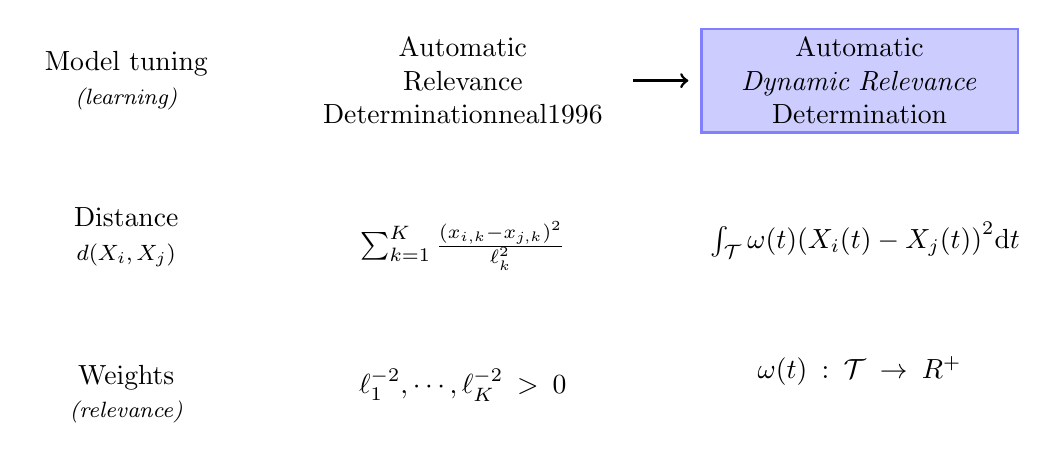
\begin{tikzpicture}
    [
    txtbox1/.style={rectangle,align=center,draw=blue!50,fill=blue!20,thick},
    every label/.style={font=\itshape\footnotesize}
    ]
    \tikzset{every node/.style={align=center}}
    \node (aspect1b)   at (0, 0)                        [text width=15ex] {
      Model tuning\\{\footnotesize \itshape (learning)}
    };
    \node (aspect2)    [below=of aspect1b]              [text width=15ex] {
      Distance\\{\footnotesize $d(X_i, X_j)$}
    };
    \node (aspect3)    [below=of aspect2]               [text width=15ex] {
      Weights\\{\footnotesize \itshape (relevance)}
    };
    %%%%%
    \node (solution1b) [right=of aspect1b]              [text width=25ex] {
      Automatic\\Relevance\\Determination\citep{neal1996}
    };
    %%%%%
    \node (solution2b) [txtbox1] [right=of solution1b]  [text
    width=25ex]
    [visible on=<2->]{
      Automatic\\\textit{Dynamic Relevance}\\Determination
    };
    %%%%%
    \node (eq1b) [below=of solution1b] [text width=25ex] {
      $\sum_{k=1}^K \frac{{(x_{i, k} - x_{j, k})}^2}{\ell_k^2}$
    };
    \node (eq2b) [below=of solution2b] [text width=25ex]
    [visible on=<3->]{
      $\int_{\mathcal{T}}
      \omega(t)
      {\left(X_i(t) - X_j(t) \right)}^2 \mathrm{d}t
      $
    };
    %%%%%
    \node (par1b) [below=of eq1b] [text width=25ex]{
      $\ell^{-2}_1, \cdots, \ell^{-2}_K > 0$
    };
    \node (par2b) [below=of eq2b] [text width=25ex]
    [visible on=<4->]{
      $\omega(t): \mathcal{T} \to \mathbb{R}^+$
    };
    \draw[shorten >=1ex,shorten <=1ex,line width=1pt]
    [visible on=<2->] [->] (solution1b.east) -- (solution2b.west);
    % \draw[shorten >=1ex,shorten <=1ex,line width=1pt]
    % [visible on=<3->] [->] (eq1b.east) -- (eq2b.west);
    % \draw[shorten >=1ex,shorten <=1ex,line width=1pt]
    % [visible on=<4->] [->] (par1b.east) -- (par2b.west);
  \end{tikzpicture}
  \begin{exampleblock}{}<3->
    Risk of overfitting with as many $\ell_k$ as $K$
  \end{exampleblock}
\end{frame}

% \begin{frame}
%   \frametitle{Permutation Dynamic Feature Importance}
%   \framesubtitle{}

%   From PFI to PDFI
% \end{frame}

\section{Asymmetrical Laplace function}
\standout{Asymmetrical Laplace function\\\textsc{fiGP-ALF}}

\begin{frame}
  \frametitle{Functional Input Gaussian Process (fiGP)}
  \framesubtitle{Asymmetrical Laplace function}

  \begin{figure}[h!]
	\centering
    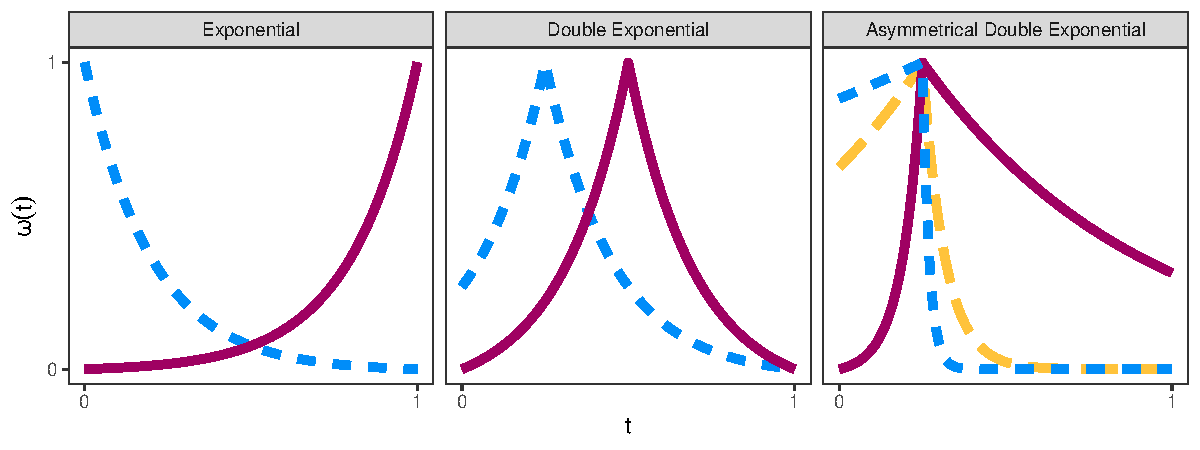
\includegraphics[width=.7\textwidth]{02-alf-weight-plot}%
  \end{figure}
  \begin{center}
    $\omega(t) = \text{exp}\left\{-(t - \tau) \lambda \kappa^s s\right\}$\\
    $\tau \sim \textsc{Beta}$,
    $\lambda \sim \textsc{N}^{+}$,
    $\log(\kappa) \sim \textsc{N}$
  \end{center}

  \blankfootnote{
    $\omega(t): \mathcal{T} = [0, 1] \to (0, 1]$,
    $s = \text{sign}(t - \tau)$,
    $\tau > 0$,
    $\lambda > 0$,
    $\kappa > 0$
  }
\end{frame}

\begin{frame}
  \frametitle{Case study}
  \framesubtitle{NASA's Microwave Limb Sounder}

    \begin{columns}[t]
    \begin{column}{0.5\textwidth}
      \begin{center}
	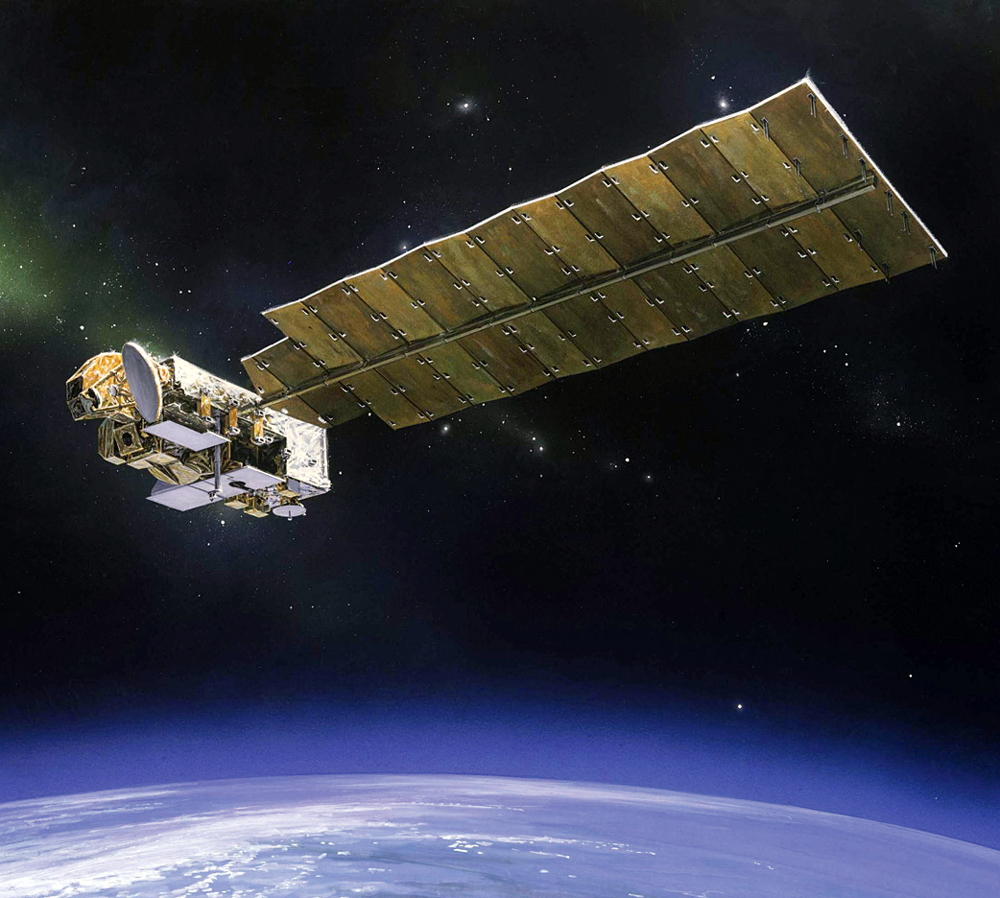
\includegraphics[height=.4\textheight]{aura.jpg}

	{\footnotesize \textit{Credit: NASA Aura}}

	\vspace{5ex}

	\definecolor{bright-spark}{RGB}{255, 195, 59}
	\tikzstyle{nice-rectangle} = [rectangle, rounded corners,
	minimum width=3cm, minimum height=1cm, text centered,
	fill=bright-spark, font=\sffamily]
	\tikzset{every label/.style={font=\itshape\footnotesize}}
	\begin{tikzpicture}
	  \node (input) [nice-rectangle] [text width = 15ex] [label=below:Functional
	  input $X(t)$] {Atmospheric constituents};
	  \node
	  (output) [nice-rectangle, right=of input]
	  [label=below:Scalar output $y$] {Radiance};
	  \draw [->] (input) [above] -- node {$f$} (output);
	\end{tikzpicture}
      \end{center}
    \end{column}
    \begin{column}{0.5\textwidth}
      \begin{tikzpicture}[overlay, remember picture]
	\node[anchor=north west] (b) at (-.2, .9) {
	  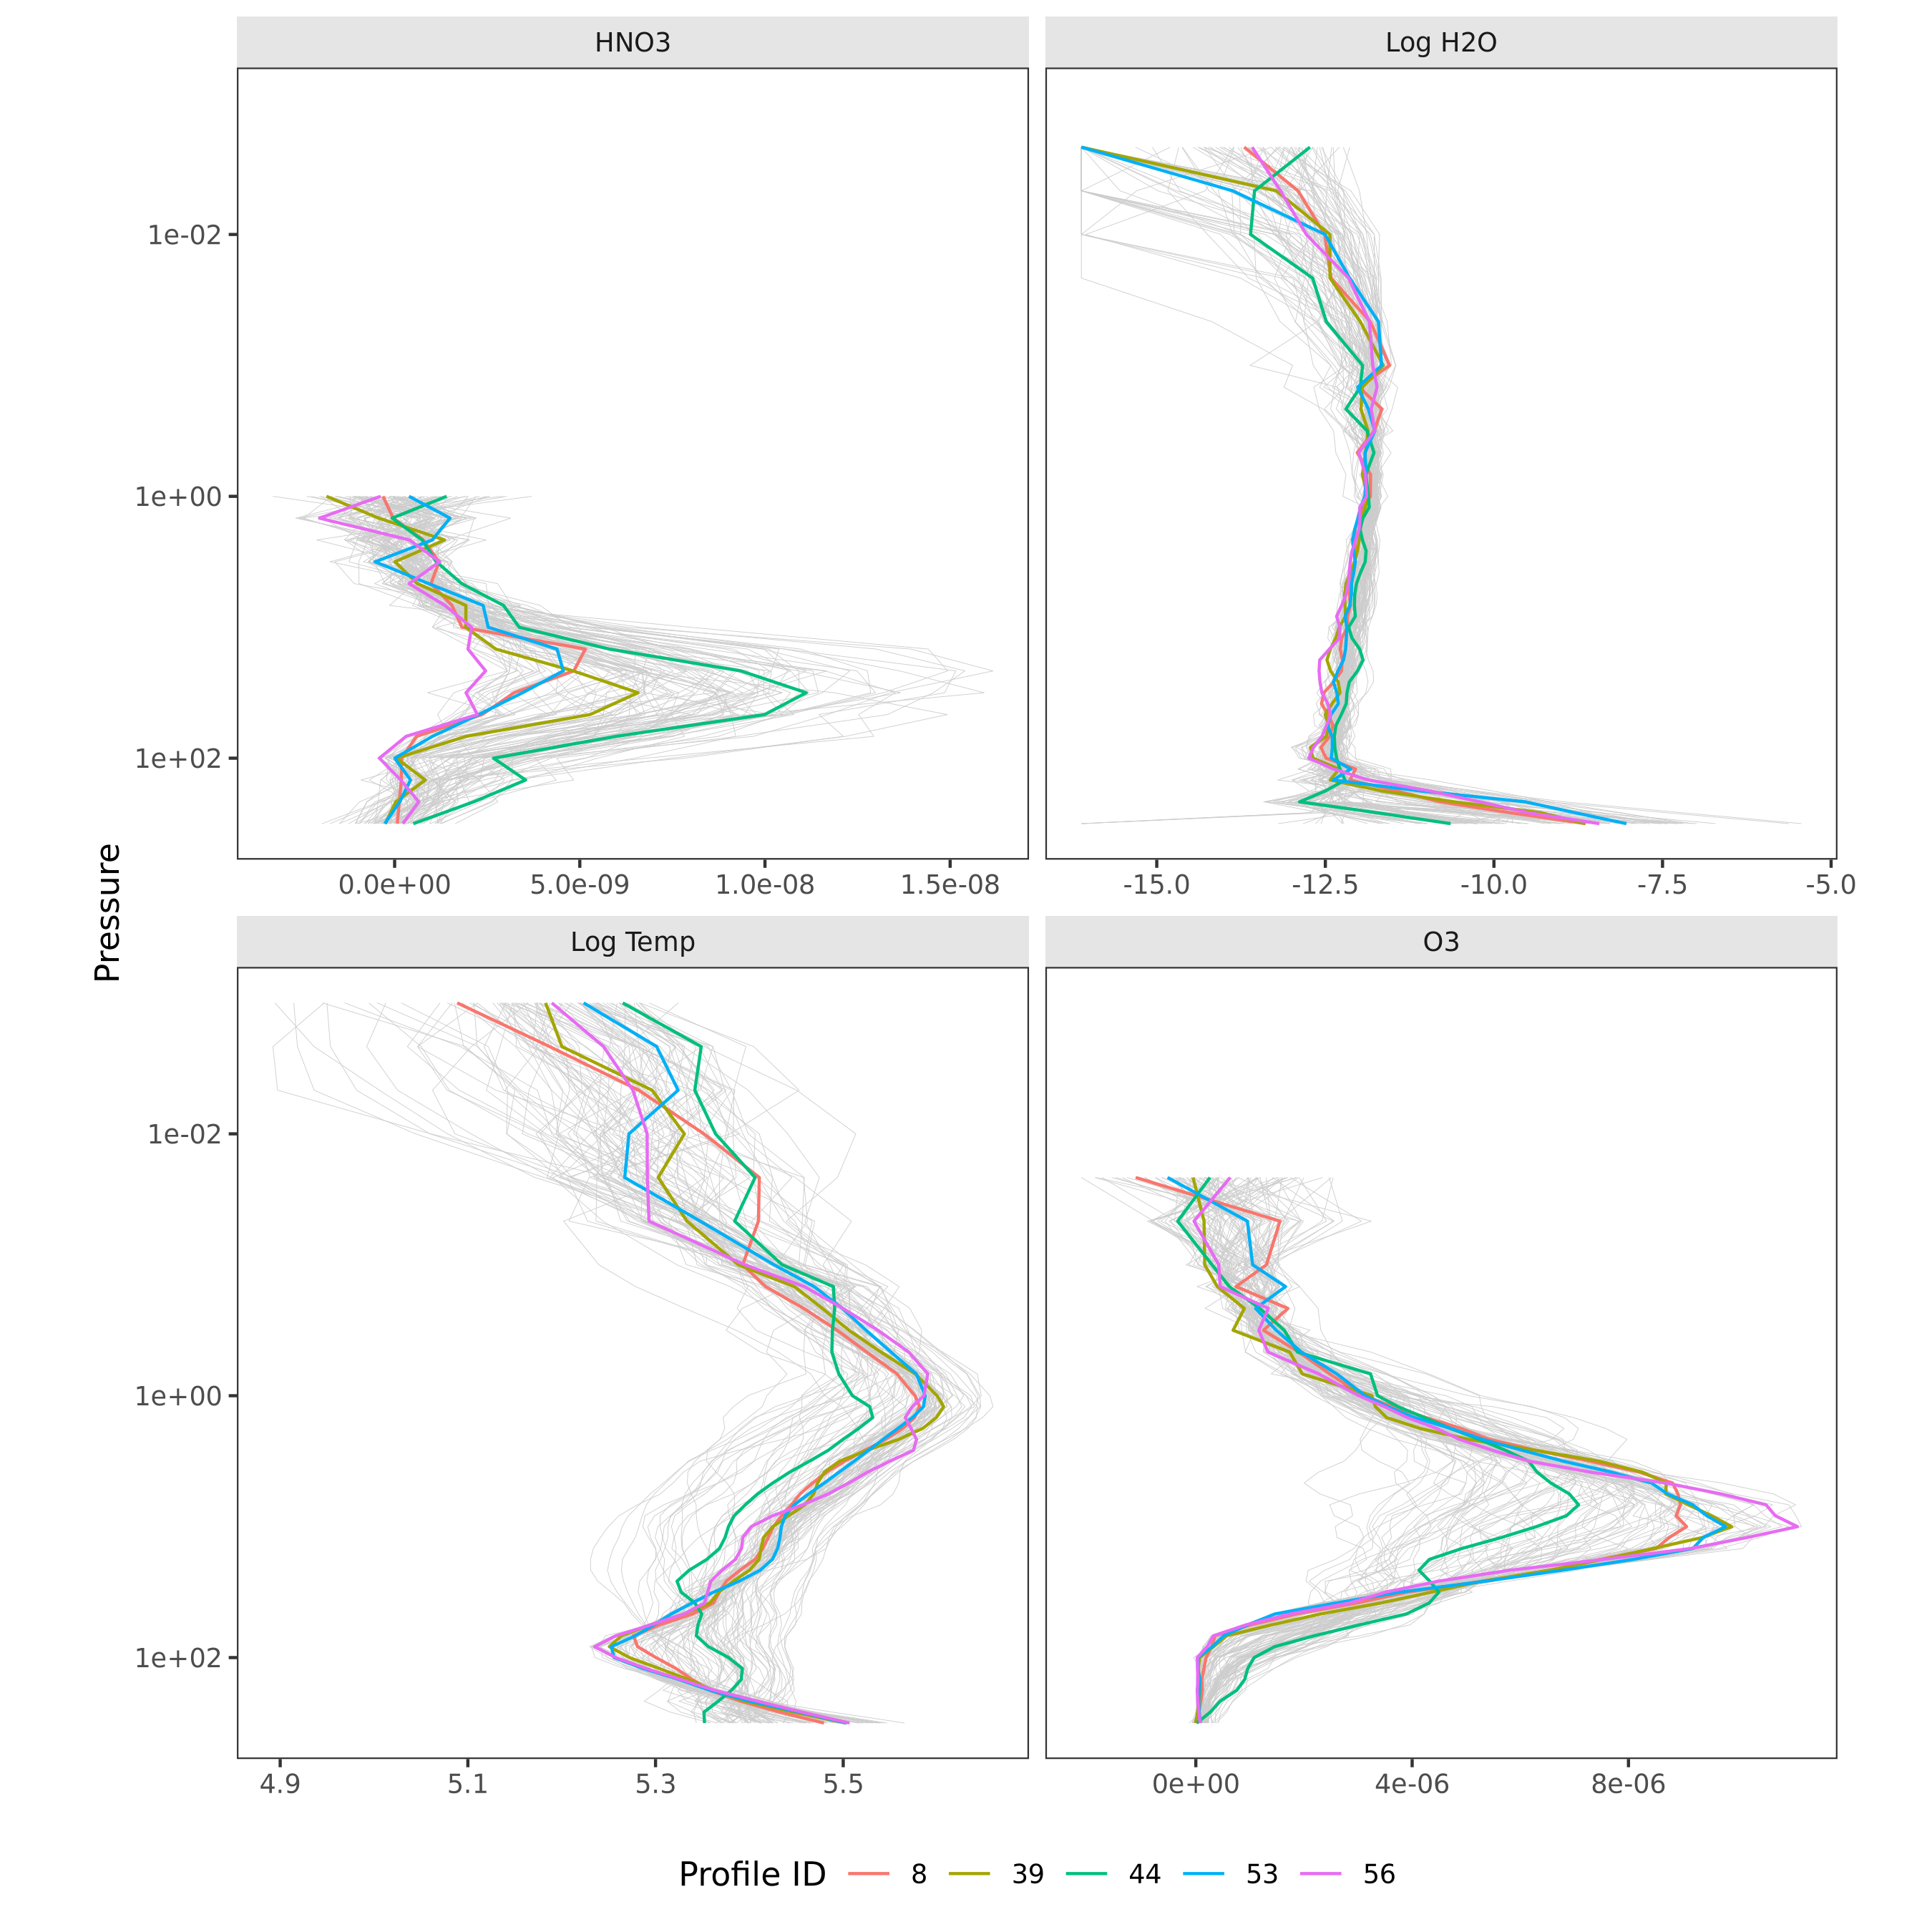
\includegraphics[height=.9\textheight]{eda-profile.png}
	};
      \end{tikzpicture}
    \end{column}
  \end{columns}
\end{frame}

\begin{frame}
  \frametitle{Case study}
  \framesubtitle{Implementation}

  \begin{itemize}
  \item 8 training and 8 test complementary sets with 1,000 soundings each
  \item 7 plausible models
    \begin{itemize}
    \item viGP SE, ARD, FPCA, FFPCA
    \item fiGP Edn, SDE, ADE
    \item One model fit separately per input-output pair
    \end{itemize}
  \item Fully Bayesian inference
    \begin{itemize}
    \item Hamiltonian Monte Carlo~\citep[ch. 5]{brooks2011}
    \item NUTS algorithm~\citep{hoffman2014} via Stan~\citep{Stan221}
    \item 1 long chain~\citep{raftery1992}
    \item Extensive search for an initial value
    \item 500 post-warmup iterations
    \item 1,500 posterior samples
    \end{itemize}
  \item Several out-of-sample validation statistics
  \end{itemize}
\end{frame}

\begin{frame}
  \begin{figure}
    \centering
    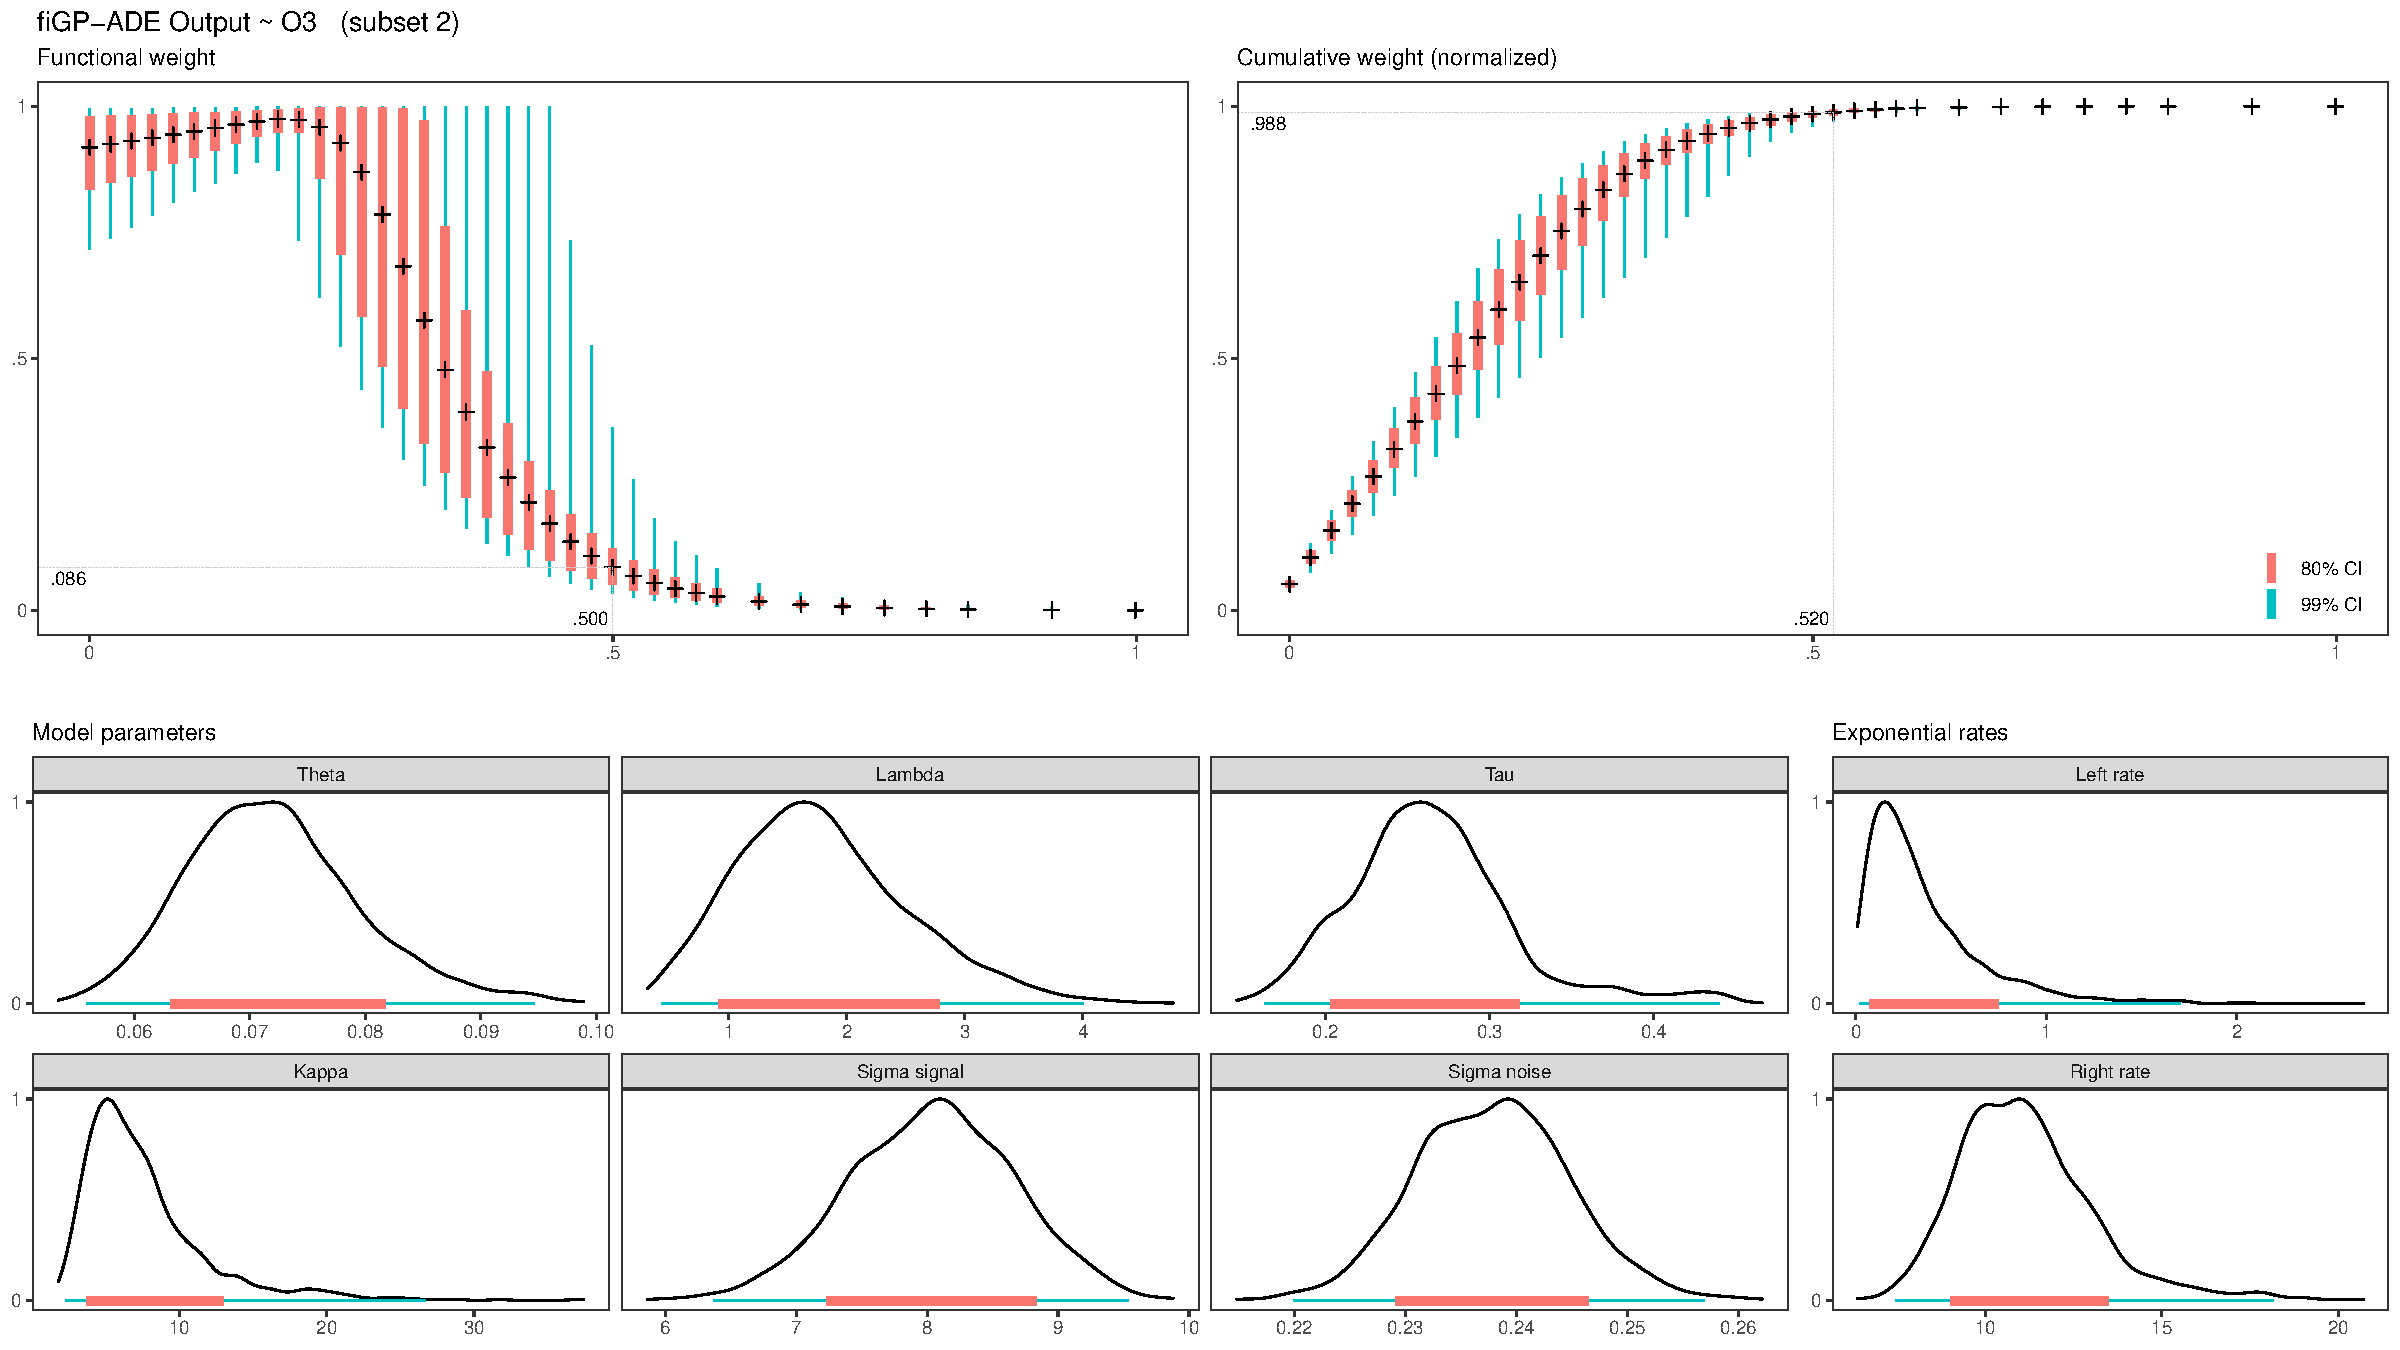
\includegraphics[width=.95\textwidth]{param-band2-unk-2-fiGP-ADE-1-O3.pdf}
  \end{figure}
\end{frame}

\begin{frame}
  \begin{figure}
    \centering
    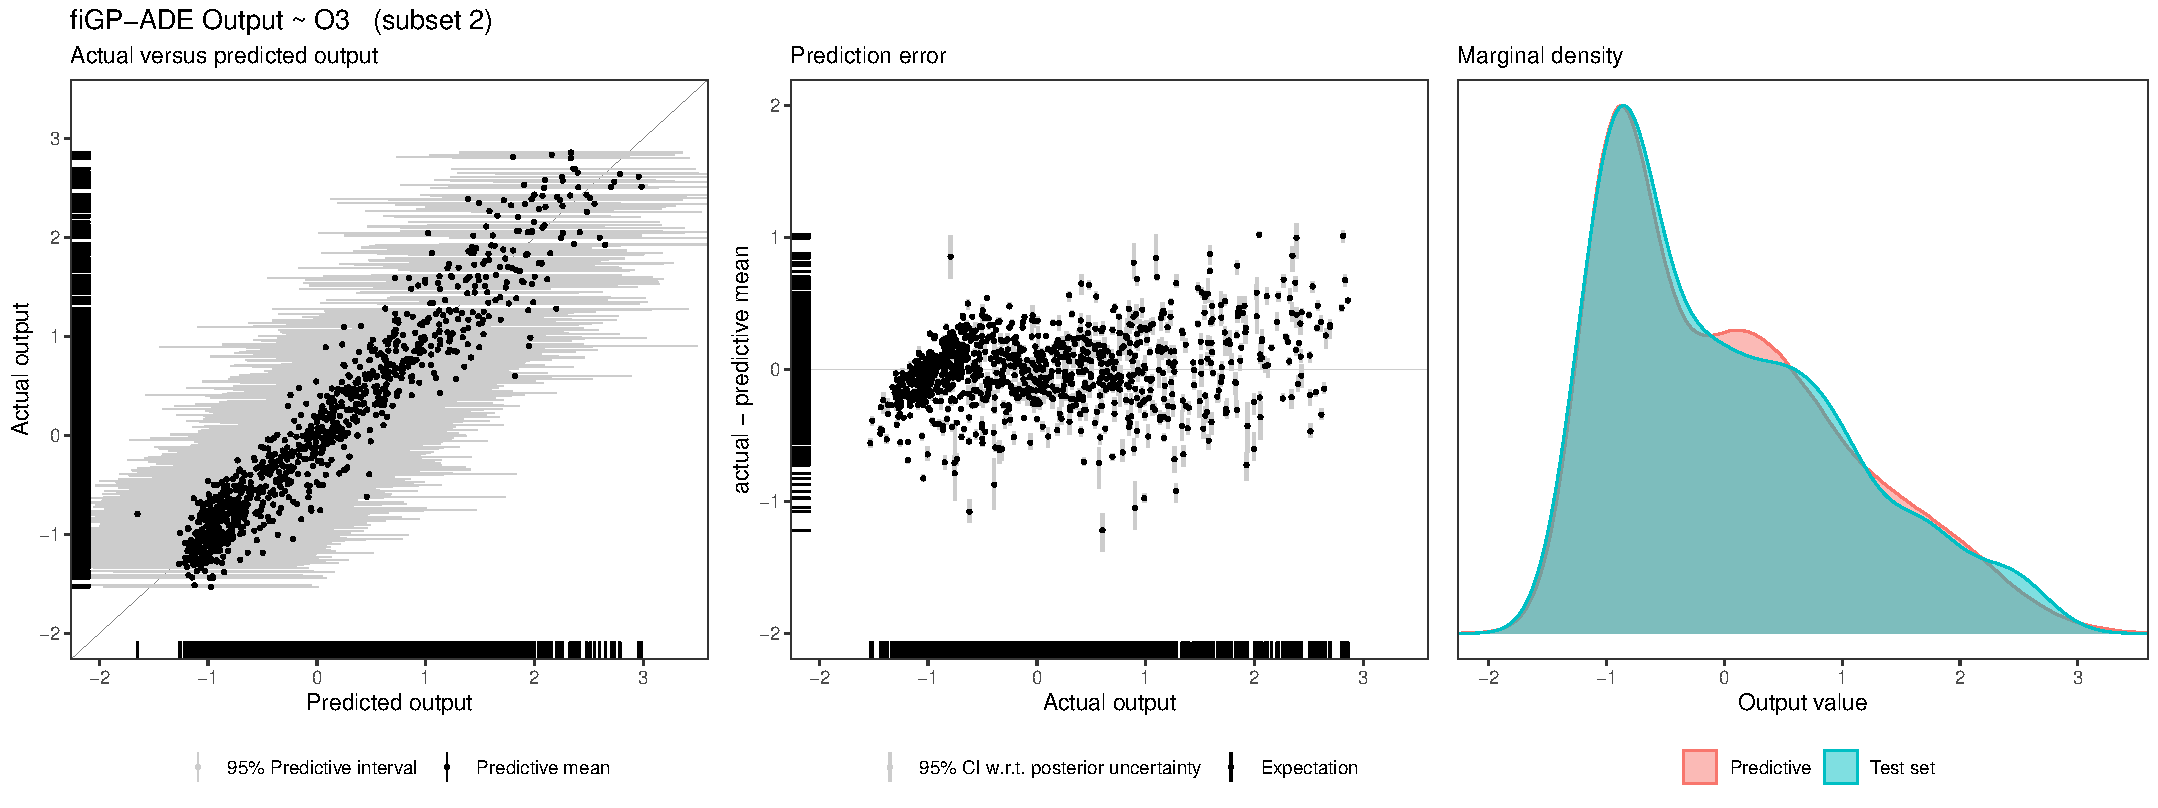
\includegraphics[width=.75\textwidth]{pred-band2-unk-2-fiGP-ADE-1-O3.pdf}
    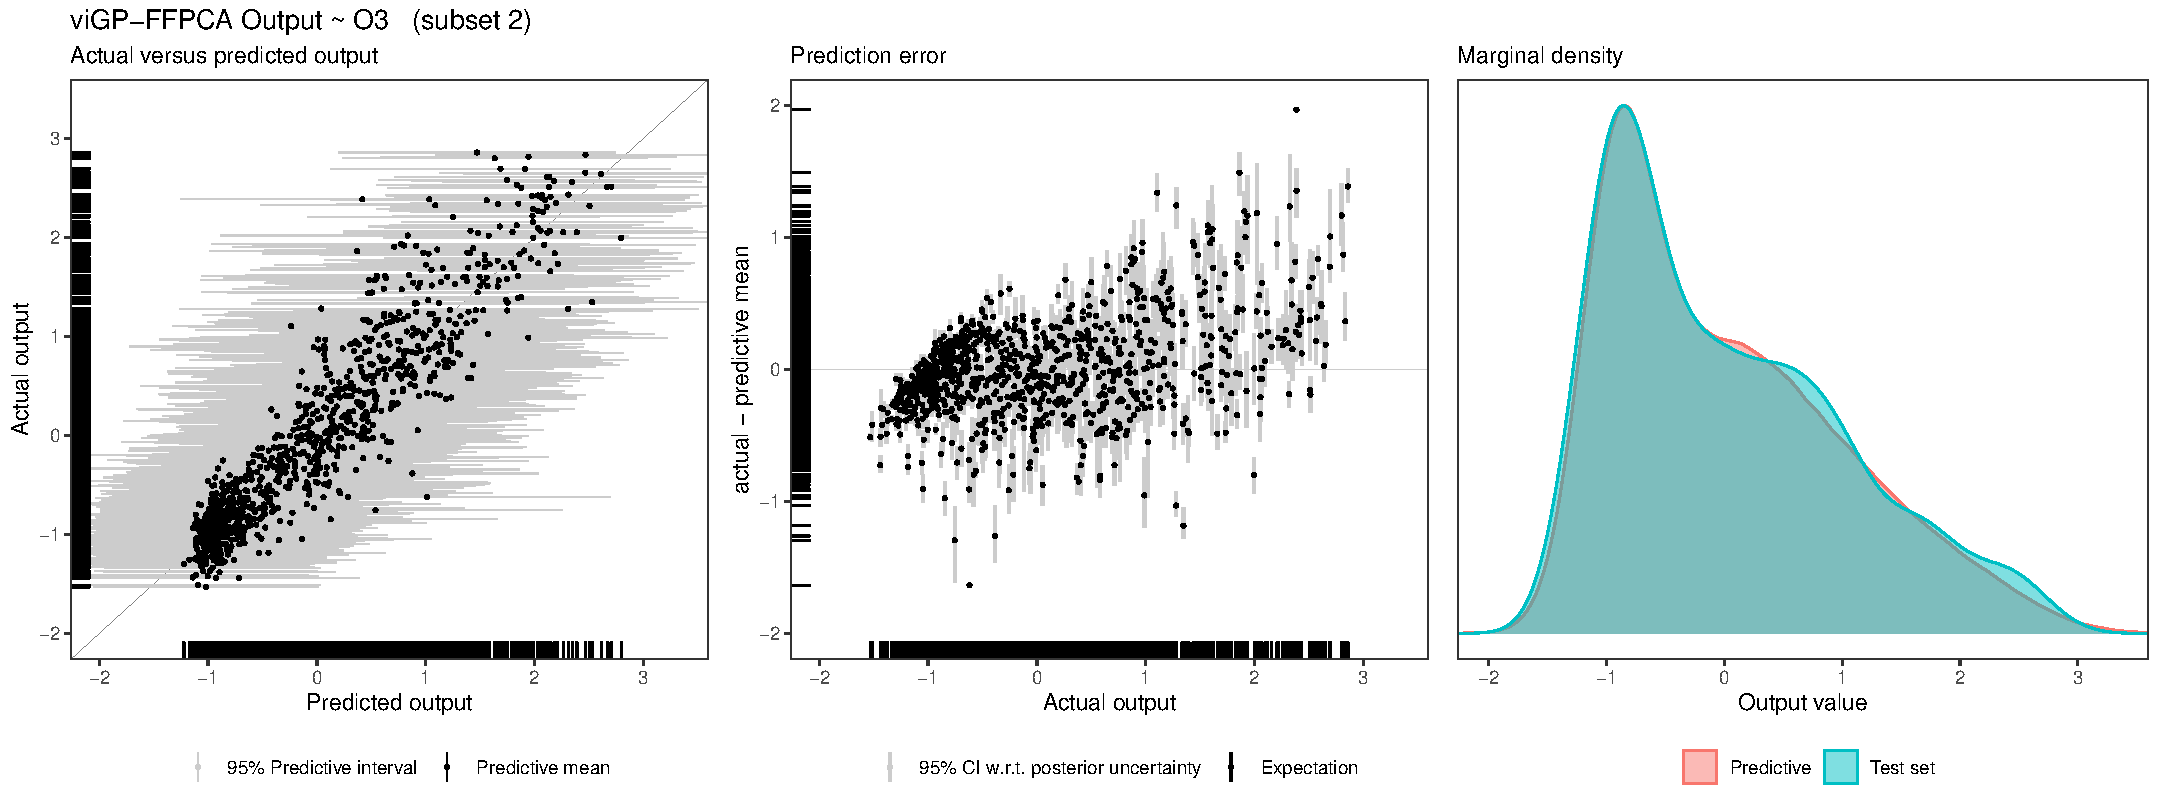
\includegraphics[width=.75\textwidth]{pred-band2-unk-2-viGP-FFPCA-1-O3.pdf}
  \end{figure}
\end{frame}

\begin{frame}
  \begin{figure}
    \centering
    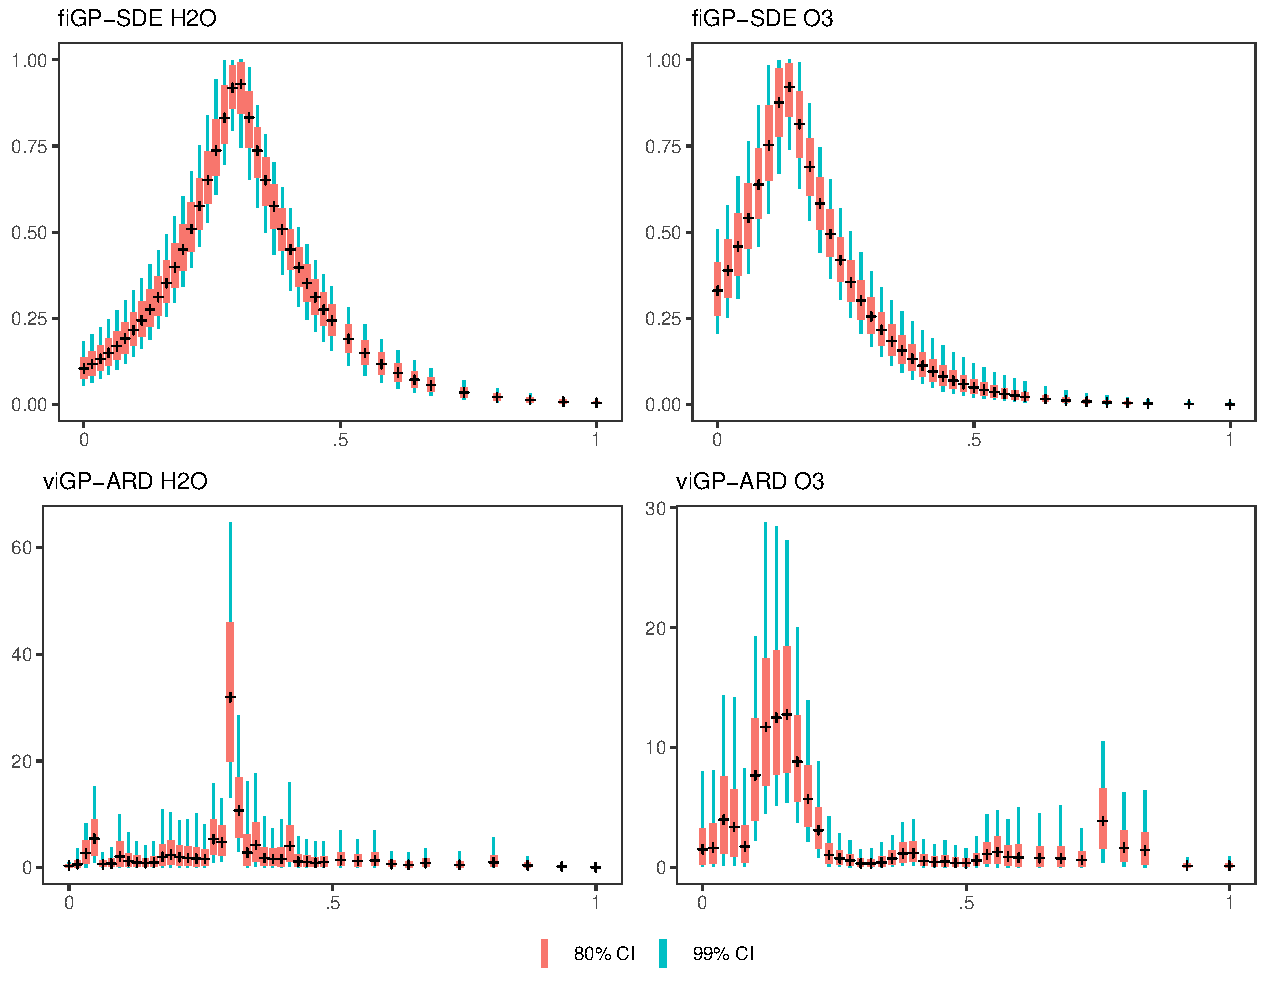
\includegraphics[height=.95\textheight]{weights-examples-pressure.pdf}
  \end{figure}

  \blankfootnote{In this slide only, we fix $\kappa = 1$ so that
    $\omega(t)$ is symmetrical}
\end{frame}

\begin{frame}
  \frametitle{Case study}
  \framesubtitle{Weight function posterior samples}

  \begin{figure}
    \centering
    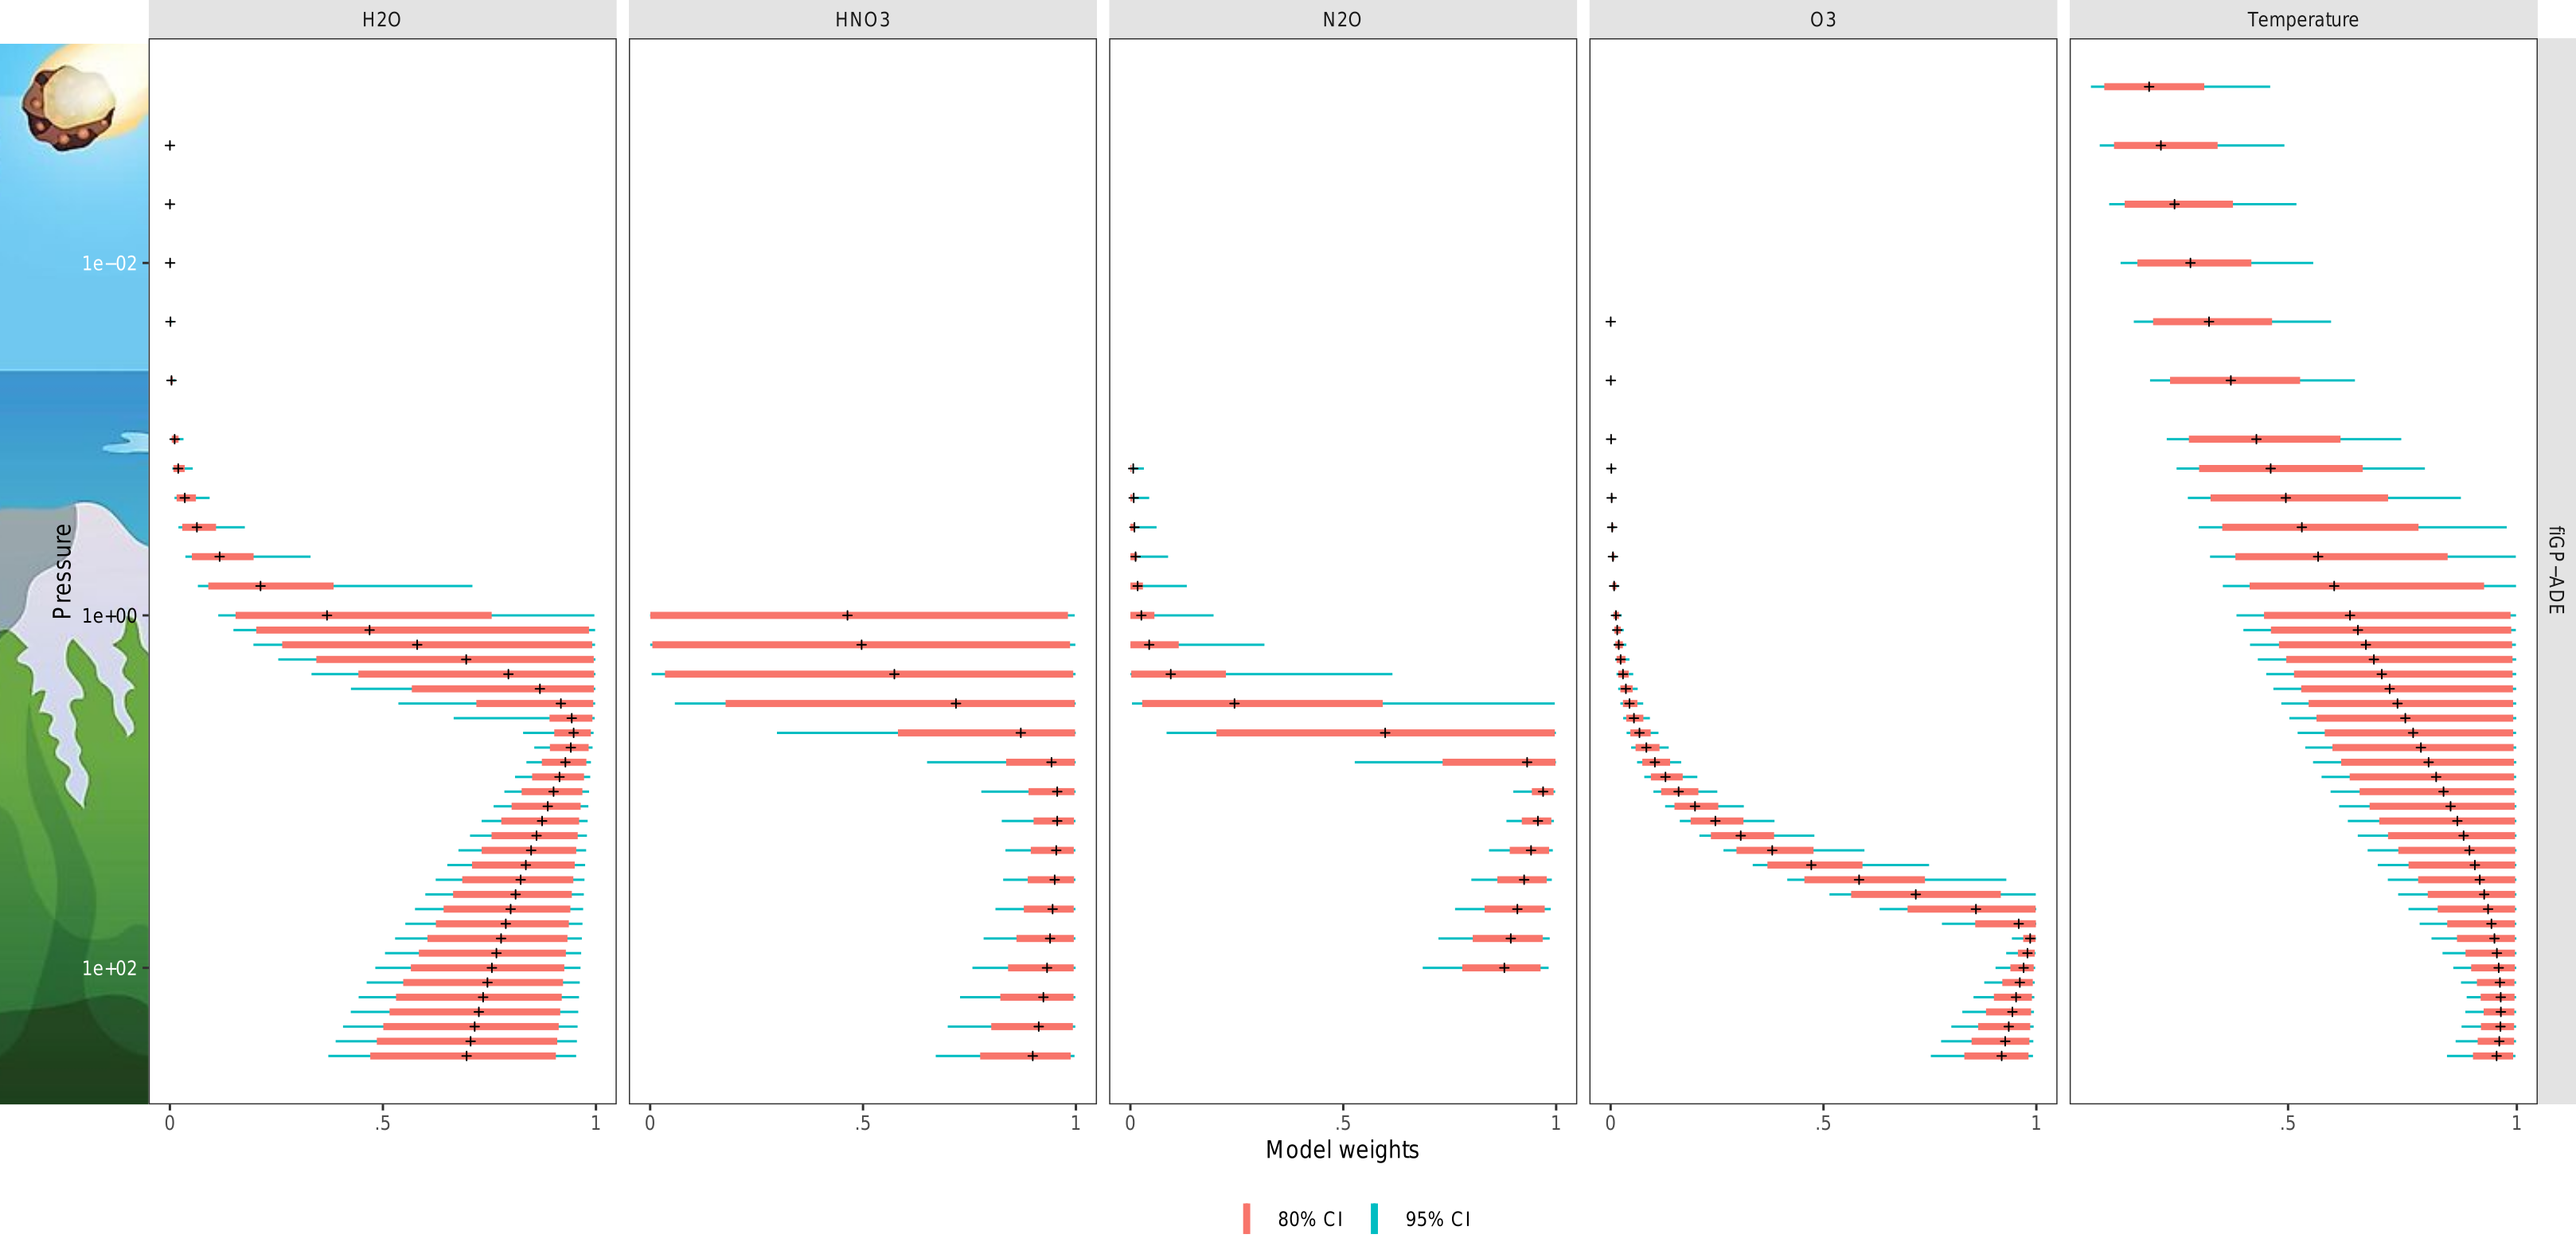
\includegraphics[width=1\textwidth]{image2934-8.png}
  \end{figure}
\end{frame}

\begin{frame}
  \frametitle{Why a fiGP?}
  \framesubtitle{In summary}

  \begin{itemize}
  \item[+]<1-> High dimensional inputs with no dimension reduction
    \begin{itemize}
    \item Reduce unknowns $3 << K$
    \item Scales up for applications with higher input resolution
      $\uparrow K$
    \end{itemize}
  \item[+]<2-> Explicit link between output correlation and
    input functional structure
    \begin{itemize}
    \item<2-> Can incorporate domain-specific knowledge
    \item<2-> Tangible for prior elicitation
    \item<2-> Interpretation $\to$ insight?
    \item<2-> Smooths out erratic relevance patterns
    \end{itemize}
  \item[+]<3-> Similar predictive power as viGP, but better than FPCA, in the
    case study
  \item[++]<4-> Extensible to \alert{\textbf{complex
        index spaces}}, e.g., spatio-temporal spectral inputs
  \end{itemize}
\end{frame}

% Chapter 2 --------------------------------------------------------------------
\section{Fourier expansion of the weights}
\standout{Fourier expansion of the weights\\\textsc{fiGP-FEW}}

\begin{frame}
  \frametitle{Fourier expansion for the weight function}
  \framesubtitle{Model specification}

  \begin{align}
  \log\omega(t)
  \label{eq:few-log}
  &=\psi_{c,0} + \sum_{g = 1}^{G} \psi_{c,g}\cos\left(2\pi gt\right)
    + \sum_{g = 1}^{G} \psi_{s,g}\sin\left(2\pi gt\right),
  \end{align}

  \begin{center}
    $\psi_{c,g},\psi_{s,g}\in\Reals$, $G\in\mathbb{N}$
  \end{center}

  \vfill{}

  \begin{itemize}[<+(1)->]
  \item Identifiability: (i) $\phi = 1$, (ii) $\psi_{c,0} = 0$,
    (iii) $\max_\mathcal{T}\omega(t) = 1$, or (iv)
    $\int_\mathcal{T}\omega(t)\dx{t} = 1$
  \item Model selection: fix $G$, or\dots
  \item Regularization priors $\psi_g\sim\mathcal{N}(0,
    g^{-2}\sigma^2_\psi)$, $\sigma_\psi\sim\mathcal{C}^+(0, 1)$
    inspired on~\citep{carvalho2010}
  \end{itemize}
\end{frame}

\begin{frame}
  \frametitle{Fourier expansion for the weight function}
  \framesubtitle{Some examples
    \hyperlink{frm:FEW-G1-span}{\beamerbutton{see more}}
  }

  \begin{figure}
    \centering
    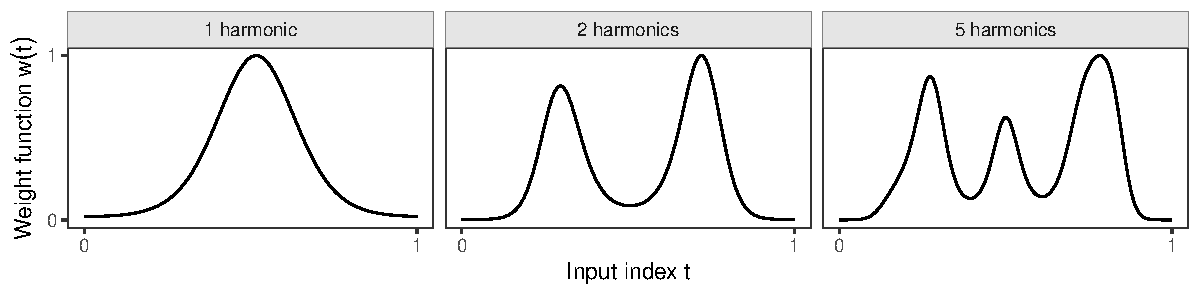
\includegraphics[width=1\textwidth]{syn01-weight-span}
  \end{figure}

  \begin{center}
    $\bm{\psi}_{c} = (-1.9, -2, -1.3, -.1, -.5)$\\
    $\bm{\psi}_{s} = (-.2, -.2, 0, .2, .1)$\\
    $G\in\{1, 2, 5\}$
  \end{center}
\end{frame}

\begin{frame}
  \frametitle{Simulation study}
  \framesubtitle{Generative models}

  \begin{figure}
    \centering
    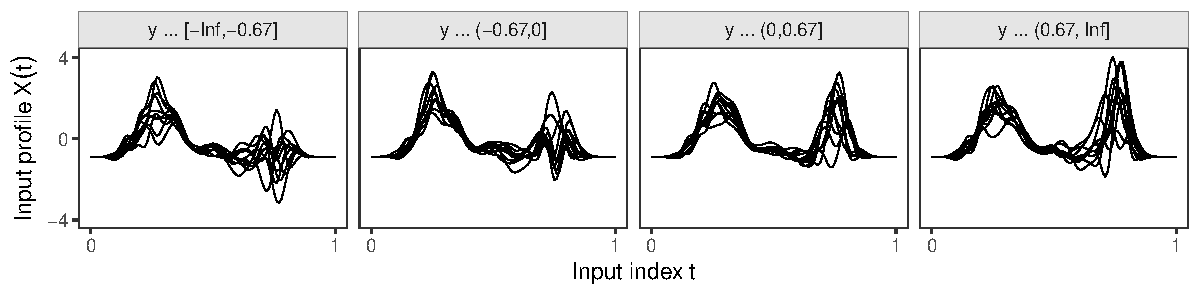
\includegraphics[width=\textwidth]{inc/syn01-inputs}
  \end{figure}

  \begin{itemize}
  \item $X(t)\sim\mathrm{GP}(m_x(\cdot), S_x(\cdot))$ calibrated to MLS O$_3$
    inputs
  \item $f^\star = \int_0^1 \sqrt{\omega(u)}\,X(u)\,\mathrm{d}u$
  \item $f = \left\{
      f^\star - \EV{f^\star}
    \right\} \VV{f^\star}^{-\frac{1}{2}}$
  \item $Y = f + \varepsilon$,
    where ${10}^{-1}\varepsilon\sim\mathcal{N}(0, 1)$
  \end{itemize}
\end{frame}

\begin{frame}
  \frametitle{Simulation study}
  \framesubtitle{True weight functions
    \hyperlink{frm:simulation-true}{\beamerbutton{see more}}
  }

  \begin{figure}
    \centering
    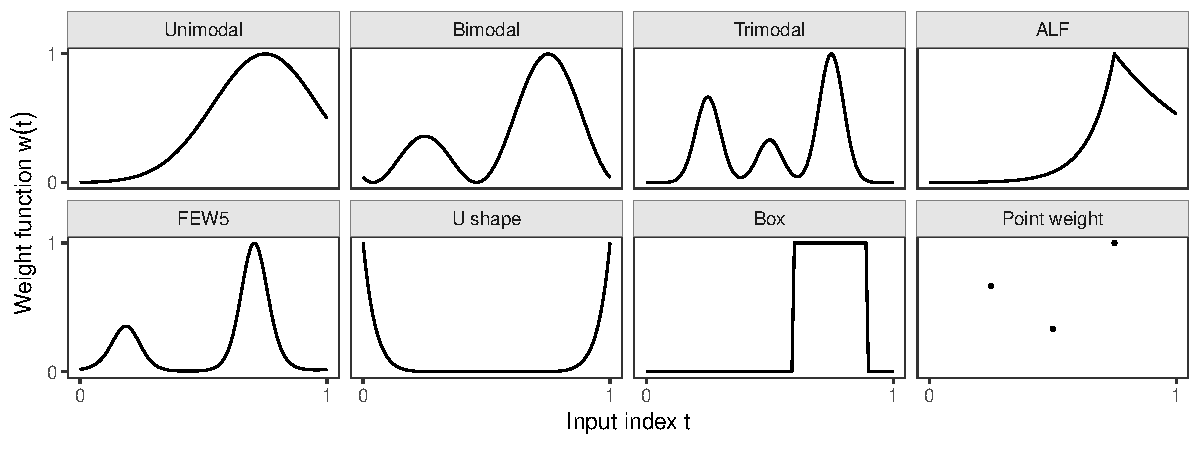
\includegraphics[width=1\textwidth]{syn01-weight-true}
  \end{figure}
\end{frame}

\begin{frame}
  \frametitle{Simulation study}
  \framesubtitle{Implementation}

  \begin{itemize}
  \item 1 training and 1 test complementary sets with 625 soundings each
  \item 8 plausible models
    \begin{itemize}
    \item viGP SE, ARD, FPCA, FFPCA
    \item fiGP ADE, FEW3, FEW5, FEW11
    \end{itemize}
  \item Research questions
    \begin{itemize}
    \item ALF and FEW vs the world
    \item Does FEW avoid overfitting as $K\to\infty$?
      $K = 10, 20, 40, 80, 160, 320$
    \end{itemize}
  \item Fully Bayesian inference (as before)
  \item Several out-of-sample validation statistics
    \hyperlink{frm:validation}{\beamerbutton{see more}}
  \end{itemize}
\end{frame}

\begin{frame}
  \frametitle{Simulation study}
  \framesubtitle{Limitations}

  \begin{itemize}
  \item It introduces strong regularization in the length-scale over the index
    space
  \item enforces periodicity and, consequently, $\omega(0) = \omega(1)$
  \item exponential function has some subtle effects
  \end{itemize}

\end{frame}

\section{Better basis functions}
\standout{Better basis functions\\\textsc{fiGP-???}}

\begin{frame}
  \frametitle{Functional Input Gaussian Process (fiGP)}
  \framesubtitle{Better basis functions}
  Early results suggest that Fourier basis are nice but limited

  Concepts to explore:
  \begin{itemize}
  \item Partition of unity of a topological space $\mathcal{T}$ is a set of
    continuous functions from $\mathcal{T}\to[0, 1]$ s.t.
  \item Wavelets
  \item Bernstein polynomials and Bézier curves
  \item Nonnegative B-splines
  \end{itemize}
\end{frame}

\begin{frame}
  \frametitle{Functional Input Gaussian Process (fiGP)}
  \framesubtitle{A likely candidate}

  Expanding nonnegative functions via splines with nonnegative coefficients

  For some knots $0 \le t^\star_0 < t^\star_1 < \dots, t^\star_n \le 1$
  \begin{align}
    \omega(t)
    &=\sum_{g=1}^{G}\psi_{g}b_g(t) \\
    b_g(t)
    &= \\
    B_{g,}
  \end{align}
\end{frame}

% Lose ends --------------------------------------------------------------------
\standout{Short notes}
\section{Loose ends}

\begin{frame}
  \frametitle{Analytical solution to piece-wise linear inputs}
  \framesubtitle{Jotting a few equations}

  \newcommand{\calT}{\mathcal{T}}
  \newcommand{\dt}{\, \mathrm{d}t}
  \newcommand{\du}{\, \mathrm{d}u}
  \newcommand{\dv}{\, \mathrm{d}v}
  \newcommand{\w}{\omega}
  \newcommand{\dotsq}{{\left[d(t)\right]}^2}
  \newcommand{\fall}{\,~\forall~\,}

  Let $\w(t): \calT \to \mathbb{R}_0^+$ be a weight function and
  $X_i(t), X_j(t): \calT \to \mathbb{R}$ be two functional inputs over
  an index space $\calT$.  Define $d_{ij}(t) = X_i(t) - X_j(t)$.  We
  want to find $ \delta_{ij} \coloneqq \int_{\calT} \w(t) \,
  {\left[d_{ij}(t)\right]}^2 \dt$. Call $f(t) \coloneqq \w(t) \,
  {\left[d_{ij}(t)\right]}^2$.  We set $\calT = [0, 1]$ and consider the
  integral over the index space for any partition $T = \left\{ t_k: t_0
    = 0 \le t_1 < \cdots < t_K \le t_{K+1} = 1 \right\}$.  We drop the
  subindexes $i$, $j$ for readability. We approach this integrals in
  three ways.
  \begin{align}
  %%% Direct integration
  \intertext{Direct integration}
  \delta
  &=\int_0^1 \w(t) \, \dotsq \dt \label{eq:fnorm-direct} \\
  &=\sum_{k = 1}^{K + 1}
    \underbrace{
    \int_{t_{k-1}}^{t_k} \w(t) \, \dotsq
    \dt}_{C_k} \label{eq:fnorm-direct-pw} \\
  %%% Integration by part 1
    \intertext{integration by parts with $u = \w(t)$ and
    $\dv = \dotsq\dt$, integration by parts with $u = \dotsq$ and $\dv =
    \w(t)\dt$}\nonumber
  \end{align}
\end{frame}

\begin{frame}
  \frametitle{Non-stationary Log-Gaussian Cox process for source separation}
  \framesubtitle{Summer internship at LANL CCS-6}
  \begin{figure}
    \centering
    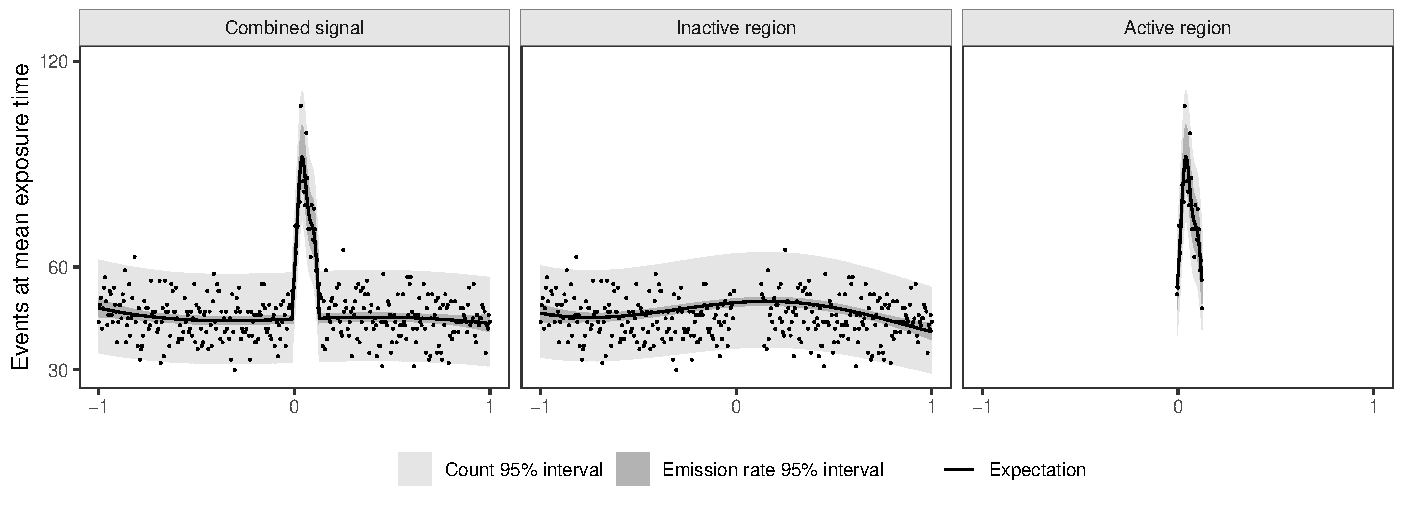
\includegraphics[width=\textwidth]{inc/application-fit-separation3.pdf}%
  \end{figure}
  {\footnotesize
    From combined to separate signals (separation)
    \begin{description}
    \item[GDF] Lower counts, very slowly moving signal
    \item[Ribbon] Higher counts, possibly rougher, inactive in most regions
    \end{description}
  }
\end{frame}

% Closing slide ----------------------------------------------------------------
\begin{frame}[c]
  \frametitle{Acknowledgments}
  \centering

  {\small Jarad Niemi, Max D. Morris\\
    Margaret Johnson (JPL), Joaquim Texeira (JPL) \\
    Microwave Limb Sounder team (JPL)\\
    David Osthus (LANL), Brian Weaver (LANL) \\
    ISU PIRI on C-CHANGE:~Science for a Changing Agriculture\\
    Foundation for Food and Agriculture Research}

  \vfill

  {\huge Thank you!}

  \vfill

  {\tiny References and extra slides on the back}

  \href{ldamiano@iastate.edu}{\beamergotobutton{mail}
    ldamiano@iastate.edu}

  \href{https://luisdamiano.github.io/}{\beamergotobutton{site}
    luisdamiano.github.io}

  \vfill

  {\tiny Am I candidate enough?}

\end{frame}

% Appendix ---------------------------------------------------------------------
\appendix

\section{References}

\setbeamertemplate{bibliography item}{\insertbiblabel}

\begin{frame}[allowframebreaks]{References}
  \tiny
  \bibliographystyle{unsrt}
  \bibliography{references}
\end{frame}

\begin{frame}
  \frametitle{Literature review}
  \framesubtitle{}
  
  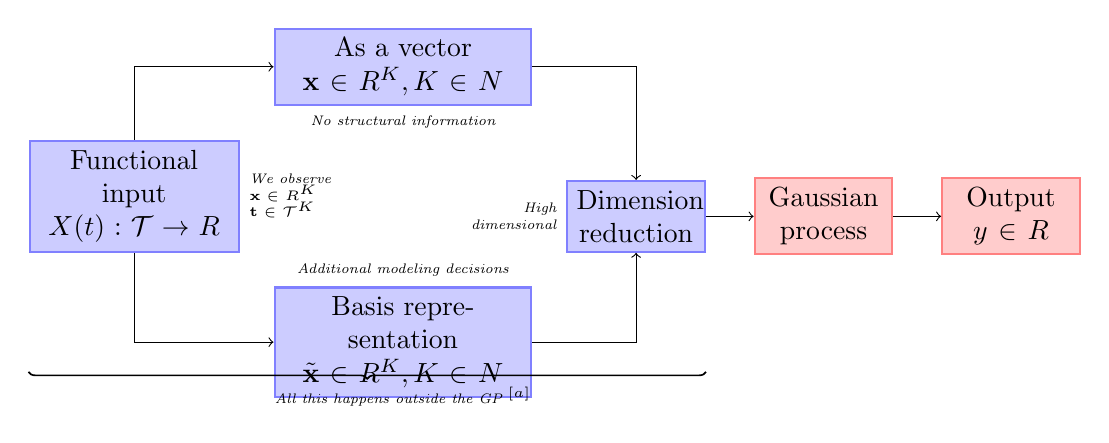
\begin{tikzpicture}
    [
    txtbox1/.style={rectangle,align=center,draw=blue!50,fill=blue!20,thick},
    txtbox2/.style={rectangle,align=center,draw=red!50,fill=red!20,thick},
    every label/.style={font=\itshape\tiny}
    ]

    \node (inp)  [txtbox1] at ( 0,  0) [text width=16ex]
    [label={[align=left]right:We observe \\ $\mathbf{x} \in \mathbb{R}^K$\\ $\mathbf{t}\in\mathcal{T}^K$}] {
      Functional input \\
      $X(t): \mathcal{T} \to \mathbb{R}$
    };
    \visible<2->{
      \node (vec1) [txtbox1] [above right=4ex of inp]   [text width=20ex]
      [label=below:No structural information]{
	As a vector \\
	$\mathbf{x} \in \mathbb{R}^K, K \in \mathbb{N}$
      };
      \node (vec2) [txtbox1] [below right=4ex of inp]   [text width=20ex]
      [label=above:Additional modeling decisions]{
	Basis representation \\
	$\tilde{\mathbf{x}} \in \mathbb{R}^K, K \in \mathbb{N}$
      };
    }
    \visible<3->{
      \node (dred) [txtbox1] [above right=4ex of vec2] [text width=10ex]
      [label={[align=right]left:High\\dimensional}]
      {
	Dimension \\ reduction
      };
    }

    \node (gp)   [txtbox2] [right=4ex of dred] [text width=10ex] {
      Gaussian \\ process
    };
    \node (out)  [txtbox2] [right=4ex of gp] [text width=10ex]  {
      Output \\ $y \in \mathbb{R}$
    };
    \visible<5->{
      \node [below=6ex of vec2.north, label=below:All this happens outside the GP$~^{[a]}$] {
      };
    }
    \draw [->] [visible on=<2->] (inp.north) |- (vec1.west);
    \draw [->] [visible on=<2->] (inp.south) |- (vec2.west);
    \draw [->] [visible on=<3->] (vec1.east) -| (dred.north);
    \draw [->] [visible on=<3->] (vec2.east) -| (dred.south);
    \draw [->] [visible on=<3->] (dred.east) -- (gp.west);
    \draw [->] (gp.east)   -- (out.west);
    \path [visible on=<5->] (inp.south west)
    edge[decorate,decoration={brace,mirror,raise=10ex},line width=.6pt]
    (inp.south west -| dred.south east);
  \end{tikzpicture}

  {\small
    \begin{itemize}
    \item<4-> Can we connect the functional input structure to a physical
      mechanism?
    \item<5-> Can we incorporate the functional input structure into the GP?$~^{[b]}$
    \item<6-> Can we circumvent input dimension reduction?
    \end{itemize}
  }

  \blankfootnote{\visible<5->{
      $~^{[a]}$\cite{muehlenstaedt2017,nanty2016,wang2017,tan2019,wang2019,betancourt2020,betancourt2020a,li2021} \,
      $~^{[b]}$\cite{morris2012,kuttubekova2019}
    }}
\end{frame}

\begin{frame}
  \frametitle{Functional input Gaussian processes}
  \framesubtitle{Validation statistics}

  \newcommand{\predmean}{\hat{\mathbf{m}}^{y}_*}
  \newcommand{\predvar}{\hat{\mathbf{S}}^{y}_*}
  \newcommand{\postpred}{\hat{p}^{y}_*}

  \begin{itemize}
  \item   Let
    $\hat{\mathbf{m}} = \predmean = \{\hat{m}_{*n}: n = 1, \dots, N\} =
    \EV{\mathbf{y}_* | \mathbf{y}, \mathbf{X}, \mathbf{X}_*}$
    and
    $\hat{\mathbf{S}} = \predvar = \VV{\mathbf{y}_* |
      \mathbf{y}, \mathbf{X}, \mathbf{X}_*}$
    be the predictive mean vector and covariance matrix.
  \item  Define the
    prediction error vector $\mathbf{e} = \mathbf{e}_{*}^{y} =
    \mathbf{y}_{*} - \hat{\mathbf{m}}$.
  \item Define the square Mahalanobis distance $D^2
    = \mathbf{e}^{\transp} \hat{\mathbf{S}}^{-1} \mathbf{e}$.
  \item Define the point-wise 95\% coverage indicator variable
    $I_{n} = 1$ if $y_{*n} \in \hat{m}_{*n} \pm 1.96
    {\hat{S}_{nn}}^{-\frac{1}{2}}$.
  \item   Let $\bar{y}_* = N^{-1} \sum_{n=1}^{N} y_{*n}$ be the test output
    mean.
  \end{itemize}

  \begin{center}
    \begin{tabular}{lrl}
      RMSE
      & $v_{\textsc{RMSE}}$ =
      & $N^{-\frac{1}{2}} \norm{\mathbf{e}}$ \\
      $R^2$
      & $v_{\textsc{R2}} $ =
      & $1 -%
        \norm{\mathbf{e}}^{2}
        \norm{\mathbf{y}_* - \bar{y}_*}^{-2}$ \\
      PPLD
      & $v_{\textsc{PPLD}}$ =
      & $
        -\frac{1}{2} \log \lvert \hat{\mathbf{S}} \rvert
        -D^2
        -\frac{n}{2} \log 2 \pi
        $
      \\
      CRPS
      & $v_{\textsc{CRPS}}$ =
      & $
        -\log \lvert \hat{\mathbf{S}} \rvert%
        -D^2
        $
      \\
      Nominal coverage
      & $v_{\textsc{COV95}}$ =
      & $N^{-1} \sum_{n = 1}^{N} I_{n}$
    \end{tabular}
  \end{center}
\end{frame}

\begin{frame}
  \frametitle{Case study}
  \framesubtitle{Out-of-sample prediction}

  \begin{table}
    \adjustbox{width=0.89\textwidth}{%
      \centering
      \begin{tabular}{lrrrrr|r}
        \toprule
        % latex table generated in R 4.0.4 by xtable 1.8-4 package
% Sat Dec 11 14:39:57 2021
%  & H2O & HNO3 & N2O & O3 & Temp & Mean \\ 
%   \midrule
% \textsc{SE} &  .34 &  .48 &  .44 &  .32 &  .25 &  .37 \\ 
%   \textsc{ARD} &  .31 &  .47 &  .43 &  .30 &  .25 &  .35 \\ 
%   \textsc{FPCA} &  .67 &  .91 &  .99 &  .46 &  .54 &  .71 \\ 
%   \textsc{FFPCA} &  .46 &  .54 &  .46 &  .38 &  .33 &  .44 \\ 
%   \textsc{Edn} &  .33 &  .47 &  .44 &  .29 &  .25 &  .36 \\ 
%   \textsc{SDE} &  .31 &  .47 &  .44 &  .29 &  .25 &  .35 \\ 
%   \textsc{ADE} &  .31 &  .47 &  .43 &  .29 &  .25 &  .35 \\ 
%    \midrule
% Mean &  .39 &  .55 &  .52 &  .33 &  .31 &  .42 \\ 
%    \bottomrule
 & H2O & HNO3 & N2O & O3 & Temp & Mean \\ 
  \midrule
  \textsc{SE}    &  .34       &  {\bf .48} &  {\bf .44} &  .32       &  {\bf .25} &  .37 \\ 
  \textsc{ARD}   &  {\bf .31} &  {\bf .47} &  {\bf .43} &  {\bf .30} &  {\bf .25} &  .35 \\ 
  \textsc{FPCA}  &  .67       &  .91       &  .99       &  .46       &  .54       &  .71 \\ 
  \textsc{FFPCA} &  .46       &  .54       &  {\bf .46} &  .38       &  .33       &  .44 \\ 
  \textsc{Edn}   &  .33       &  {\bf .47} &  {\bf .44} &  {\bf .29} &  {\bf .25} &  .36 \\ 
  \textsc{SDE}   &  {\bf .31} &  {\bf .47} &  {\bf .44} &  {\bf .29} &  {\bf .25} &  .35 \\ 
  \textsc{ADE}   &  {\bf .31} &  {\bf .47} &  {\bf .43} &  {\bf .29} &  {\bf .25} &  .35 \\ 
   \midrule
   Mean          &  .39 &  .55 &  .52 &  .33 &  .31 &  .42 \\ 
   \bottomrule
      \end{tabular}
      \begin{tabular}{lrrrrr|r}
        \toprule
        % latex table generated in R 4.0.4 by xtable 1.8-4 package
% Sat Dec 11 14:39:57 2021
  %                & H2O & HNO3 & N2O & O3 & Temp & Mean \\ 
  % \midrule
  % \textsc{SE}    & 273 & 613 & 589 & 142 & -4 & 323 \\ 
  % \textsc{ARD}   & 196 & 619 & 581 & 92 & -14 & 295 \\ 
  % \textsc{FPCA}  & 1024 & 1320 & 1406 & 637 & 802 & 1038 \\ 
  % \textsc{FFPCA} & 535 & 646 & 630 & 295 & 268 & 475 \\ 
  % \textsc{Edn}   & 260 & 623 & 585 & 90 & 4 & 312 \\ 
  % \textsc{SDE}   & 202 & 623 & 585 & 85 & 4 & 300 \\ 
  % \textsc{ADE}   & 202 & 610 & 581 & 89 & 2 & 297 \\ 
  %  \midrule
  %  Mean & 385 & 722 & 708 & 204 & 152 & 434 \\ 
  %  \bottomrule
                 & H2O & HNO3 & N2O & O3 & Temp & Mean \\ 
  \midrule
  \textsc{SE}    & 273       & {\bf 614} & {\bf 585} & 138      & {\bf -7}  & 323 \\ 
  \textsc{ARD}   & {\bf 196} & {\bf 619} & {\bf 581} & {\bf 92} & {\bf -13} & 295 \\ 
  \textsc{FPCA}  & 1024      & 1320      & 1406      & 637      & 802       & 1038 \\ 
  \textsc{FFPCA} & 535       & {\bf 646} & {\bf 630} & 295      & 268       & 475 \\ 
  \textsc{Edn}   & 261       & {\bf 623} & {\bf 585} & {\bf 90} & {\bf 4}   & 312 \\ 
  \textsc{SDE}   & {\bf 202} & {\bf 623} & {\bf 585} & {\bf 85} & {\bf 4}   & 300 \\ 
  \textsc{ADE}   & {\bf 202} & {\bf 610} & {\bf 581} & {\bf 87} & {\bf 2}   & 297 \\ 
   \midrule
   Mean & 385 & 722 & 708 & 204 & 152 & 434 \\ 
   \bottomrule
      \end{tabular}}
    \caption{Mean validation statistics
      $\bar{v}^{(p, q)}$: RMSE (left) and negPPLD (right).
      Smaller values are better. Bold: best in class.}%
    \label{tab:validation-statistics-mini}
  \end{table}

  Mean validation statistics: RMSE (left) and negative posterior
  predictive log-density (right).  Smaller values are better. Bold: best
  in column. \textsc{Edn} $\tau = 0, \kappa = 1$; \textsc{SDE} $\tau =
  0$; \textsc{ADE} $\tau, \kappa, \lambda$ all free; \textsc{ARD} as
  many free parameters as measurements per vertical profile.
\end{frame}

\begin{frame}
  \frametitle{FEW function with one harmonic}
  \framesubtitle{$\psi_{c}$ in the rows, $\psi_{s}$ in the column}

  \begin{figure}
    \centering
    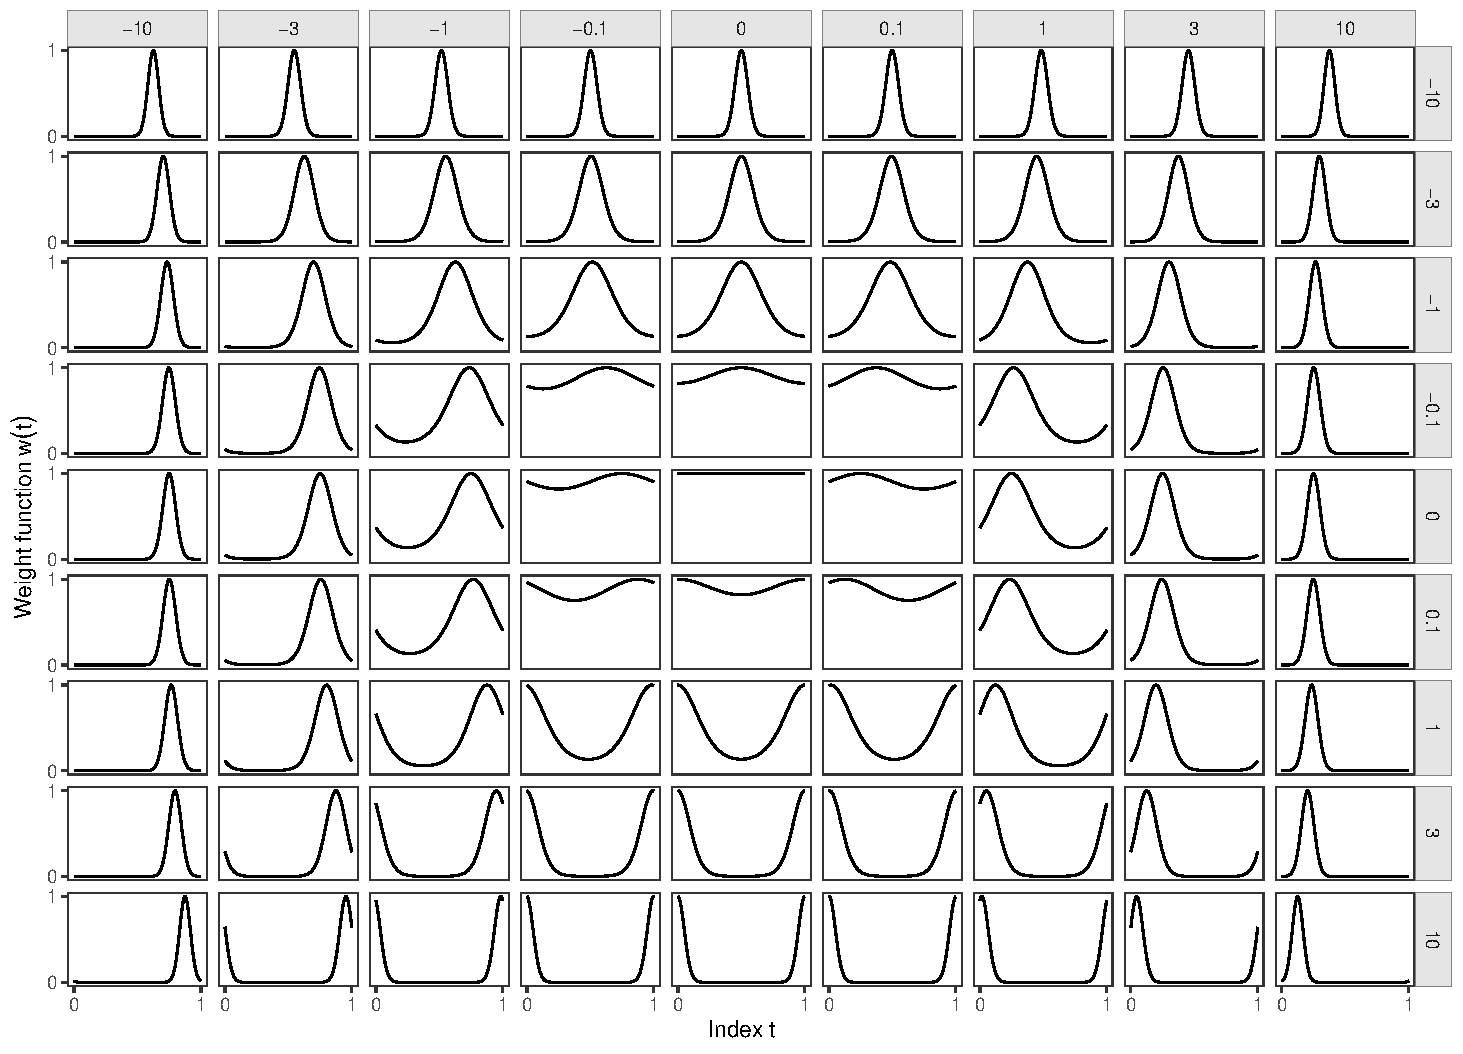
\includegraphics[width=.65\textwidth]{FEW-G1-span}
  \end{figure}
\end{frame}

\begin{frame}
  \frametitle{Simulation study}
  \framesubtitle{True weight functions}

  \vspace{-2ex}
  {\small
    \begin{align*}
      \omega^\star_1(t)
      &=Q(t, .75, .30)
      &\text{Unimodal} \\
      \omega^\star_2(t)
      &=\left\{1.13 + \sin[2\pi(1-t)] - \cos[2\pi2(1-t)]\right\} / 3.13
      &\text{Bimodal} \\
      \omega^\star_3(t)
      &=\frac{2}{3} Q(t, .25, .07)+
        \frac{1}{3} Q(t, .50, .07) +
        \frac{3}{3} Q(t, .75, .07)
      &\text{Trimodal} \\
      \omega^\star_4(t)
      &=
        \begin{cases}
          \exp\left(10\,\lvert t - .75 \rvert\right) \\
          \exp\left(-2.5\,\lvert t - .75 \rvert\right) \\
        \end{cases}
      &\text{ALF} \\
      \omega^\star_5(t)
      &=
        \begin{aligned}[t]
          &\exp\left\{\right.
          .2 +
          1/3 \cos(2\pi t) - 5/3 \cos(2\pi2t) - \\
          &2/3 \sin(2\pi t) + 4/3 \sin(2\pi2t)
          \left.\right\} / 17.62
        \end{aligned}
      &\text{FEW5} \\
      \omega^\star_6(t)
      % &= {\left(\frac{t - .5}{.5}\right)}^{10}
      &= {(2t - 1)}^{10}
      &\text{U shape} \\
      \omega^\star_7(t)
      % &=1 - \mathbb{I}(t < .9) - \mathbb{I}(t < .6)
      &=\mathbb{I}(.6\le t \le.9)
      &\text{Box} \\
      \omega^\star_8(t)
      &=\mathbb{I}(t\in\{.25, .50, .75\})
      &\text{Point mass}
    \end{align*}
    $Q(t, a, b) = \exp\left[-{(t - a)}^2/b^2\right]$, and $\mathbb{I}(\cdot)$
    is an indicator function}
\end{frame}

\end{document}

%%% Local Variables:
%%% eval: (TeX-run-style-hooks "beamer")
%%% mode: latex
%%% TeX-master: t
%%% End:
